\documentclass{standalone}
\usepackage{tikz}


\begin{document}

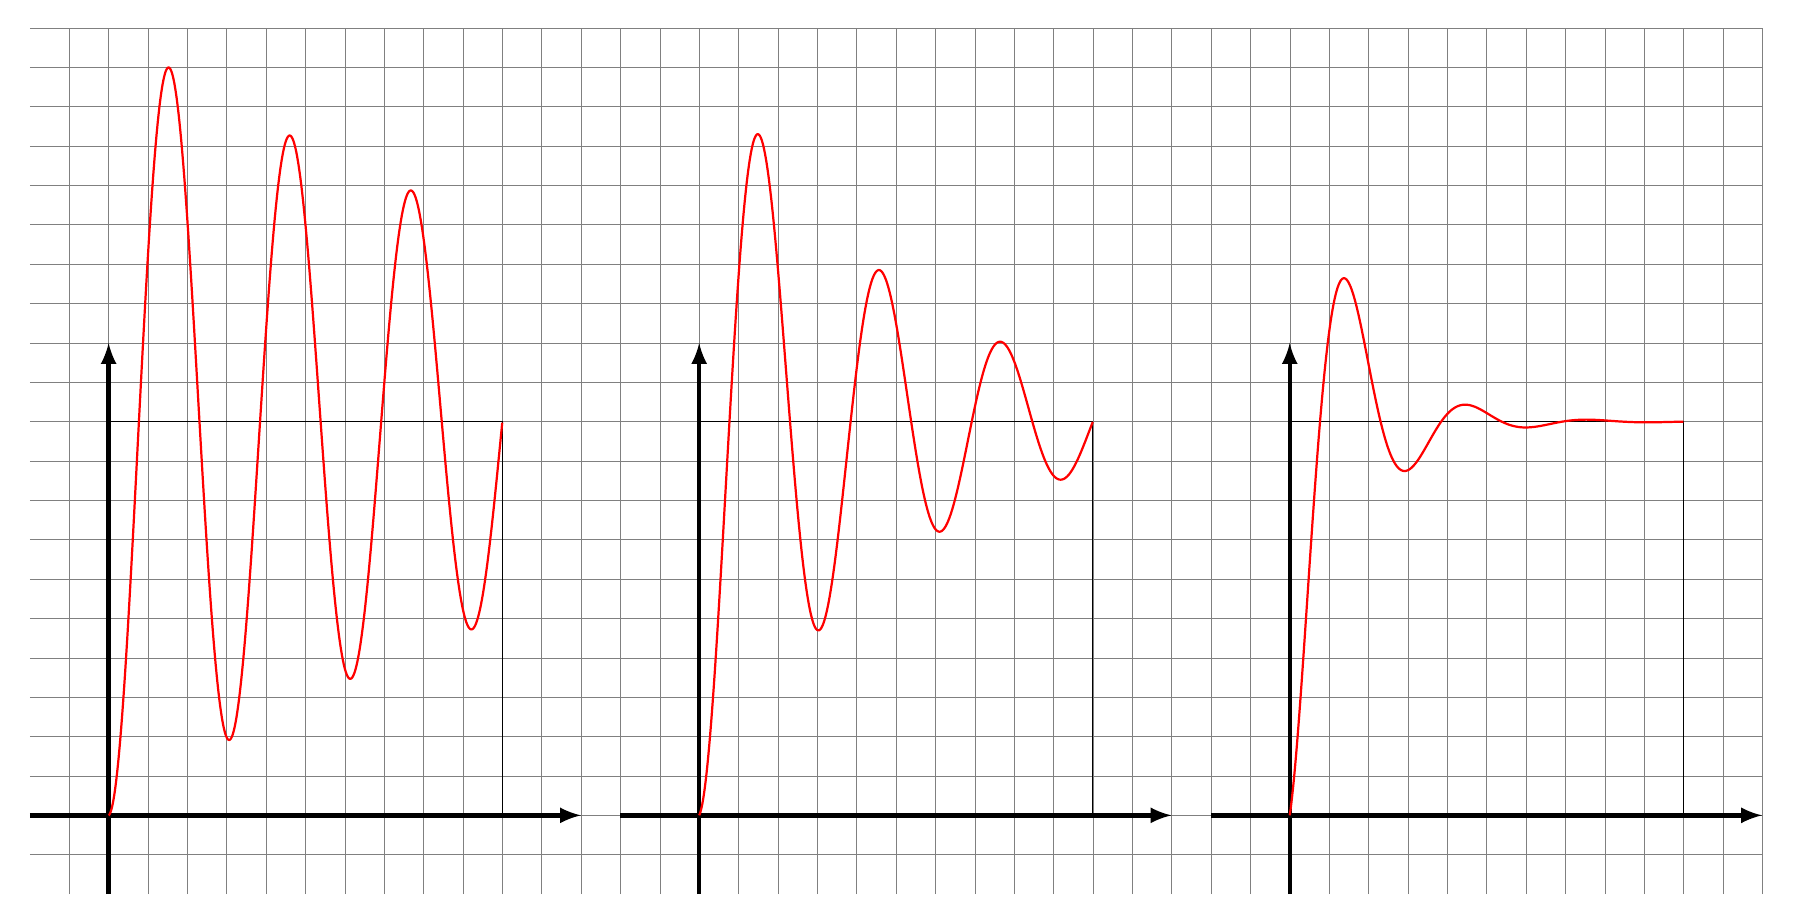
\begin{tikzpicture}[scale=5,axis/.style={-latex,ultra thick},graph/.style={red,thick}]
  \draw[help lines] (-0.2,-0.2) grid[step=0.1cm] (4.2,2);

  \begin{scope}
    \draw (0,0) rectangle (1,1);
    \draw[axis] (-0.2,0) -- (1.2,0);
    \draw[axis] (0,-0.2) -- (0,1.2);
  
  \draw[graph] plot[domain=0:1,smooth,samples=1000] (\x,{1-cos(\x*360*3.25) * 0.5^(1*\x)});
  \end{scope}

  \begin{scope}[xshift=1.5cm]
    \draw (0,0) rectangle (1,1);
    \draw[axis] (-0.2,0) -- (1.2,0);
    \draw[axis] (0,-0.2) -- (0,1.2);
  
    \draw[graph] plot[domain=0:1,smooth,samples=1000] (\x,{1-cos(\x*360*3.25) * 0.5^(3*\x)});
  \end{scope}

  \begin{scope}[xshift=3cm]
    \draw (0,0) rectangle (1,1);
    \draw[axis] (-0.2,0) -- (1.2,0);
    \draw[axis] (0,-0.2) -- (0,1.2);
  
    \draw[graph] plot[domain=0:1,smooth,samples=1000] (\x,{1-cos(\x*360*3.25) * 0.5^(10*\x)});
  \end{scope}
\end{tikzpicture}

\end{document}